\chapter{Integrated Discussion}
\label{ch:discussion}

The welding proposal asked how a process-aware multimodal architecture could be designed and evaluated for industrial anomaly detection. It called for a comparison of what the camera, acoustic signal, and machine measurements could predict about weld quality. The project moved to PHM gear monitoring and REASSEMBLE robotic assembly. When the Intel Welding data were subsequently reconsidered, the feasibility audit documented prior use of the proposed test population (Chapter~1 and Appendix~\ref{app:chronology}). That population could no longer supply an independent estimate of weld-quality performance.

Combining predictions improved failure ranking over the sensor component in REASSEMBLE assembly. The comparison used a common action outcome and held out entire recordings. In MSM milling and ViFailback manipulation, stacking ranked outcomes less accurately than its sensor component. In HANDOVER, equal averaging likewise fell below sensor-only prediction. In PHM, the interpretation of prediction error depended on how closely the photograph-derived measure corresponded to gear damage. Each comparison used the same target and held-out observations within its study. Extending the comparison to welding requires welds reserved for assessment and an independently measured quality outcome.

\section{Representation Suitability --- Answer to SQ1}
In PHM, the image-regression experiment extracted detector features during a full prediction pass. In the principal sensor experiment, post-run photographs instead supplied the continuous target. A patch-based Transformer encoded sequences summarizing speed, torque, temperature, vibration and condition indicators. For SQ1, the regression error measures how well this representation predicts the photographic proxy. Assessing physical tooth damage would require a separate reference (Chapter~5).

Across 4,530 completed REASSEMBLE actions, engineered sensor statistics achieved pooled failure average precision (AP) of .429, compared with .242 for a short-budget, scratch-trained PatchTST and .231 for a frozen convolutional image encoder with mean frame pooling (Table~\ref{tab:reassemble-unimodal}). The backbone that produced the image features was ResNet18-vd inside the pretrained RT-DETR-R18vd checkpoint. Averaging the frame features discarded their temporal order. Pooling near the action boundary improved an exploratory visual result, which is consistent with outcome cues appearing near completion. It leaves open whether the same representation would be useful before the outcome became visible. A separate two-epoch frozen versus fine-tuned comparison gave opposite visual effects across two seeds (Appendix~\ref{app:supplementary-results}). These results apply to the training budgets, patch lengths, masks, and pooling rules tested here.

In MSM, the frozen camera representation had mean AP of .299 for abnormal milling intervals. Ninety sensor statistics yielded .829 with logistic regression and .901 with histogram gradient boosting (HGB). Weak visual performance could reflect limited visibility of the event or how the frozen encoder represented it. The study did not isolate these explanations (Table~\ref{tab:msm-clean}). ViFailback pooled three camera views per episode and summarized 28 robot-observation channels. Transferring a visual encoder trained on REASSEMBLE produced mixed changes across target-training seeds relative to generic frozen features (Table~\ref{tab:vif-matched}). A newly fitted head could use the transferred features, but their predictive advantage varied across seeds.

HANDOVER provided a further test of representation on a shared observation window. Sixteen video frames and 36 force--torque statistics described the same portion of each trial. The wrench was measured on one robot and estimated from joint torques on the other. Mean failure AP was .772 for vision and .824 for logistic sensing on the official test trials (Table~\ref{tab:handover-clean}). Across the five studies, compact sensor summaries provided strong references, and frozen convolutional features supplied a reusable visual input whose value depended on the task and time window. Published acoustic representations remain candidates for the original welding objective. None of the five studies establishes which audio encoder to deploy, and the scratch-trained time-series comparisons leave the benefit of pretrained time-series weights open.

\section{Comparative Fusion Performance --- Answer to SQ2}
In PHM, concatenating the embeddings of three sensor groups gave a mean absolute error of 0.824 percentage points on the photographic proxy, compared with 0.804 for the training mean when entire experiments were held out. The paired interval allowed either model to have lower error (Table~\ref{tab:phm-loeo}). This comparison addresses sensor-feature fusion under SQ2. A separate four-arm study included an affine combination and a context gate. Its normalizer was fitted before the evaluation split loop, which compromises the isolation of held-out observations within that diagnostic. The principal leave-one-experiment-out comparison used a separate training-only normalizer.

REASSEMBLE supplied the most direct comparison of the four approaches. Across 148 held-out recordings evaluated in five folds, concatenation achieved .412 failure AP, the statistical sensor predictor .429, equal probability averaging .446, and logistic stacking (F2) .447. The original gates ranged from .441 to .445 (Tables~\ref{tab:reassemble-unimodal} and~\ref{tab:reassemble-fusion}). The paired AP difference between stacking and sensors was .0179 (95\% recording-level bootstrap CI [.0086, .0283]). Against averaging, the difference was .0016 (95\% CI [$-.0076$, .0112]). The fitted stacker ranked failures more accurately than its sensor component. The interval for stacking versus averaging included gains and losses in failure ranking.

Attributing that gain specifically to visual information requires an additional control. The stacker fitted a logistic map, with an intercept, to calibrated branch probabilities. Its sensor component had no corresponding second calibration stage. The original gates combined branch logits using constrained weights, and feature concatenation changed both the information available to the classifier and its capacity. These comparisons measure the performance of fitted systems. The later matched controls address more specific questions about how the weights were chosen.

On MSM, mean AP over three seeds was .757 for stacking, .736 for averaging, .829 for the constituent logistic sensor model, and .901 for the separate sensor HGB reference. The paired date-cluster interval for stacking minus logistic sensing was below zero, conditional on the saved fits and five dates. Figure~\ref{fig:within-study} shows the reversal of the stacking--sensor comparison between assembly and milling. ViFailback gave a similar direction for a different endpoint. Original stacking attained pooled macro-AP of .621--.629 across three seeds versus .649 for logistic sensing (Table~\ref{tab:vif-bothclass} and Chapter~8). Macro-AP here weights success and failure equally. In HANDOVER, averaging the two branch predictions gave mean failure AP of .803 on 151 official test trials, below the sensor component at .824. The missing participant-to-trial mapping prevented construction of the participant-disjoint predictions required to fit the planned stacker. HANDOVER therefore supplies a measured comparison for averaging and an open question for learned fusion. Across these tasks, the clearest gain occurred for simple prediction fusion in assembly. The two other stacking studies and the handover averaging study each favored their constituent sensor model on the primary ranking metric.

\begin{figure}[htbp]
\caption{Prediction Performance With Intact Inputs by Study}\label{fig:within-study}
\centering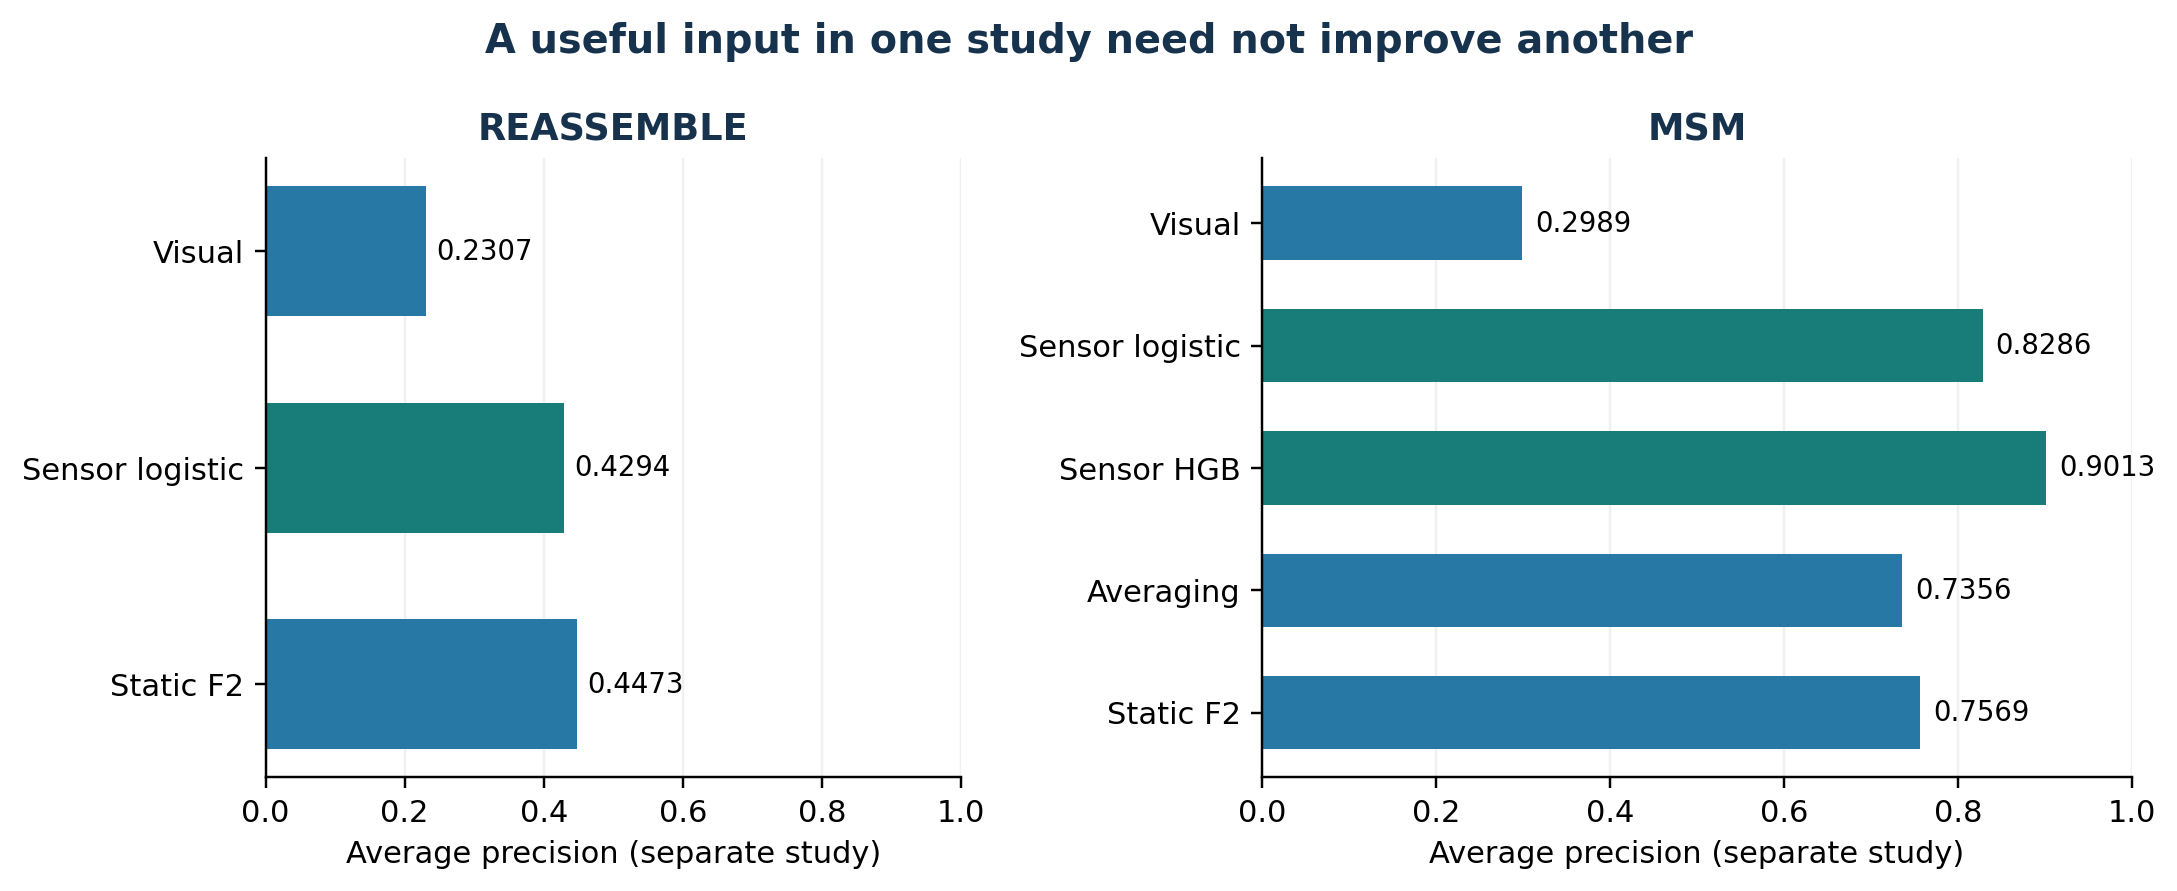
\includegraphics[width=\textwidth]{figures/within_study_results.png}
\displaynote{REASSEMBLE uses pooled failure average precision for 4,530 actions. MSM uses the mean of three seed-specific average precision scores, each calculated from pooled outer-fold predictions. The panels have different targets, prevalence, and evaluation protocols. The panel values and their sources are listed in Appendix~\ref{app:reproducibility}, \EvidenceRef{E107}{}.}
\end{figure}

\section{Robustness and Reliability --- Answer to SQ3}
SQ3 asks whether a gate improves robustness when inputs are missing, degraded, or unreliable. A known outage and a plausible but erroneous reading require different responses. PHM illustrates the distinction even within the sensor stream. In its separate four-arm diagnostic, one nominal group had no input columns, so dropping it removed no information. The gate was computed from context, so corrupting inputs to the other branches could leave its weights unchanged. Small changes around an already weak regression predictor give limited evidence about reliability. The photographs supplied the target in the principal comparison, leaving inference-time camera loss outside that experiment.\ev{PHM group dropout and conditioning}{\EvidenceRef{E004}{section 12.6}}

In REASSEMBLE, known complete loss of a stream routed the prediction to the surviving branch. Every fusion rule using that policy inherited the survivor's score. When both streams remained present and the sensor stream received Gaussian noise at one training standard deviation, stacking gave AP of .222 and the quality-only and combined gates gave .175 and .179, respectively. Intact vision alone achieved .231. Responding to noise by changing a weight therefore did not ensure a better failure ranking. The result pertains to this corruption and severity.

A later context-conditioned adjustment to the static REASSEMBLE stacker raised clean AP from .4473 to .4683. Its paired clean increment was .0210 (95\% CI [.0015, .0419]). Under matched augmentation, the mean adaptive increment over six corruption conditions was .0097 (95\% CI [$-.0034$, .0228]). A further pilot comparing a quality interaction with an exposure-matched static model also left its primary robustness increment unresolved, .0030 (95\% CI [$-.0267$, .0322]). These follow-ups support a gain for a particular adjustment on clean data. They do not show that conditioning on the measured quality variables improved decisions across degraded inputs.\ev{Distinct adaptive investigations}{\EvidenceRef{E004}{sections 18.2--18.3 and 19.5}}

In MSM, the strongest sensor noise reduced stacking to .207 AP. The augmentation-trained gate reached .299, approximately the score of intact vision alone. Under the strongest image blur, the same gate reached .683, below stacking at .771 and intact logistic sensing at .829. In HANDOVER, the strongest blur left averaging at .779 versus .824 for intact logistic sensing. Known complete loss used an explicit fallback. The participant grouping requirement prevented evaluation of a learned gate there (Appendix~\ref{app:handover}). ViFailback evaluated a clean camera-view ablation. The SQ3 corruption tests were outside its final computational budget, leaving the effect of degradation on its predictors unmeasured.

REASSEMBLE, MSM, and HANDOVER implemented a fallback to the surviving predictor when a stream was declared absent. Across the five studies, a consistent predictive gain from adaptive weighting under degraded but present inputs remains unresolved. A fair test gives the static and adaptive models the same corruption exposure and calibration opportunities, then compares each with the intact or degraded single stream available in that condition. Whether such a gate improves weld-quality decisions under sensing failures remains open.

\section{Evaluation Beyond Accuracy --- Answer to SQ4}
The PHM error measures agreement with image-derived candidate area in percentage points per run. For SQ4, interpreting that agreement as physical damage requires an independent measurement. Twenty nominal runs came from three gear experiments. Holding out a whole experiment tests whether the predictor generalizes beyond runs from experiments represented during fitting. Uncertainty estimated from saved run predictions remains conditional on the fitted models.

REASSEMBLE shows how to distinguish failure ranking, probability calibration, and the threshold at which an operator would act. The positive AP increment over sensors did not resolve every recall or calibration contrast. A review of 64 selected action clips found 57 agreements among 59 determinate judgments, with five indeterminate and two disagreements. The review exposed uncertainty about outcome visibility and boundaries. Its stratified sample and single reviewer limit population-level estimates of annotation accuracy (Appendix~\ref{app:human-review}). Recorded timings for the visual, sensor, and fusion components describe a warmed computation with prepared inputs. Operational latency also includes acquisition, completion of the observation window, and the response to a prediction.

At seed 42 in MSM, stacking had a lower Brier score than logistic sensing (.056 versus .062), even though logistic sensing ranked abnormal intervals better. In ViFailback, failure prevalence exceeded 85\%. At seed 42, stacking achieved failure AP of .945 and success AP of .312, yielding macro-AP of .629 (Table~\ref{tab:vif-bothclass}). Reporting both classes exposed a weakness that the majority-class score concealed. Task-cluster intervals characterize variation over the assessed tasks conditional on the fitted models. Session and operator dependence remain additional sources of uncertainty.

In HANDOVER, 110 of the 151 test trials were failures. At a threshold of .5, a training-prior predictor labelled every trial a failure, achieving failure F1 of .843 and zero specificity for successes. The official split remained usable for evaluating fixed baselines, while unavailable participant identifiers prevented participant-level uncertainty estimates for their contrasts. These examples support reporting prediction time, label provenance, class-specific discrimination, probability error, threshold consequences, and the grouping used for uncertainty. The branch predictions and fitted coefficients show how each stream contributed to a fused score. Establishing whether operators interpret it correctly or can act in time would require prospective observation and a usability study.

\section{Agreement and Disagreement With Previous Research}
Evidence from welding itself qualifies the expectation of a fusion advantage. In one penetration-state study, the clean image-only, audio-only, and fused models each reached 100\% accuracy \citep[Tables~1--3]{Hua2026Weld}. Distinct physical measurements may be available even when the reported endpoint leaves no measurable room for a clean gain. In the published HANDOVER study, five-class outcome accuracy averaged over five trainings was 69.1\% with video and force/torque and 67.9\% after gripper state was added \citep[Table~III]{Thoduka2024Handover}. The present HANDOVER implementation uses binary outcomes, different models, and failure AP. The common finding is that an additional stream can lower performance on a shared outcome. Absolute scores from the two experiments answer different questions.

Other industrial studies report clear gains within their respective protocols. Acoustic--thermal gearbox monitoring achieved 99.54\% mean accuracy against 90.54\% for the stronger individual thermal stream on a random within-condition split \citep[Table~2]{Ying2025Trustworthy}. On MVTec~3D-AD, combining RGB and 3D inputs raised mean image AUROC to 93.7\% from 88.0\% for RGB alone \citep[Table~3]{Rudolph2023Asymmetric}. These results concern different acquisition regimes and outcomes from completed-action failure. Conversely, studies of multimodal optimization and industrial input subsets identify losses against stronger individual channels \citep{Wang2020What,Horwitz2023Back,Goodarzi2023Deep}. REASSEMBLE and the external studies provide evidence in both directions. The performance differences alone cannot identify whether limited visibility, an unsuitable representation, or the fusion training procedure caused a particular loss.

Previous work provides both a theory and experimental tests of quality-aware weighting \citep{Zhang2023QMF}. RGB--geometry research tests absent 3D input \citep[Table~3]{P026}, and fuzzy-regularized camera--telemetry fusion tests corruption in simulated robot pose regression \citep{Altinses2023Fuzzy}. Training-time removal of images, a model designed for single-stream inference, an unannounced sensor malfunction, and adaptation with target-domain data impose different information constraints. The remaining question for a particular industrial task is whether a quality signal changes decisions beneficially once the static and unimodal controls have comparable observations, calibration, and training exposure.

\section{Lessons Across Datasets and Limits of Comparison}
Table~\ref{tab:cross-study} returns to the main research question. The units range from gear runs to individual actions, milling intervals, manipulation episodes, and handovers. Within each study, the single-input and fused models can be compared directly. Differences in targets, observation windows, class frequencies, and splits preclude a common ranking across datasets.

\begin{table}[htbp]
\caption{Interpretation of the Results Within Each Study}\label{tab:cross-study}
\centering\small

\begin{tabularx}{\textwidth}{P{27mm}YYY}
\toprule Study & Target/unit & Supported lesson & Principal boundary\\\midrule
PHM & Photo-derived proxy per gear run & Three sensor groups gave no clear improvement over the training mean & Physical damage reference unavailable\\
REASSEMBLE & Completed action failure & Stacking improved on sensors. Equal averaging performed similarly & Extra calibration step in stacking\\
MSM & Abnormal milling interval & Sensor models ranked abnormal intervals more accurately than stacking & Five dates in the paired interval\\
ViFailback & Whole-episode outcome & Original stacking fell below logistic sensing. Encoder transfer had mixed effects & Target-CNN adaptation and corruption tests deferred\\
HANDOVER & Success or failure of a handover trial & Averaging improved on vision alone but fell below logistic sensing & Participant grouping for learned fusion unresolved\\\bottomrule
\end{tabularx}
\displaynote{Each effect applies to the evaluation protocol for its study.}
\end{table}

MSM and HANDOVER reused a visual feature extractor and refitted predictors to their local targets. ViFailback additionally tested parameters learned on REASSEMBLE by fitting fresh heads on the transferred features. Reusing a procedure, transferring learned weights, and deploying an unchanged predictor on a new physical installation each require different evidence. Figure~\ref{fig:gap-coverage} locates the completed comparisons within the literature synthesis. The accompanying matrix identifies the studies and the comparisons underlying each question.
\begin{figure}[htbp]
\caption{Literature Comparisons and Experimental Coverage}\label{fig:gap-coverage}
\centering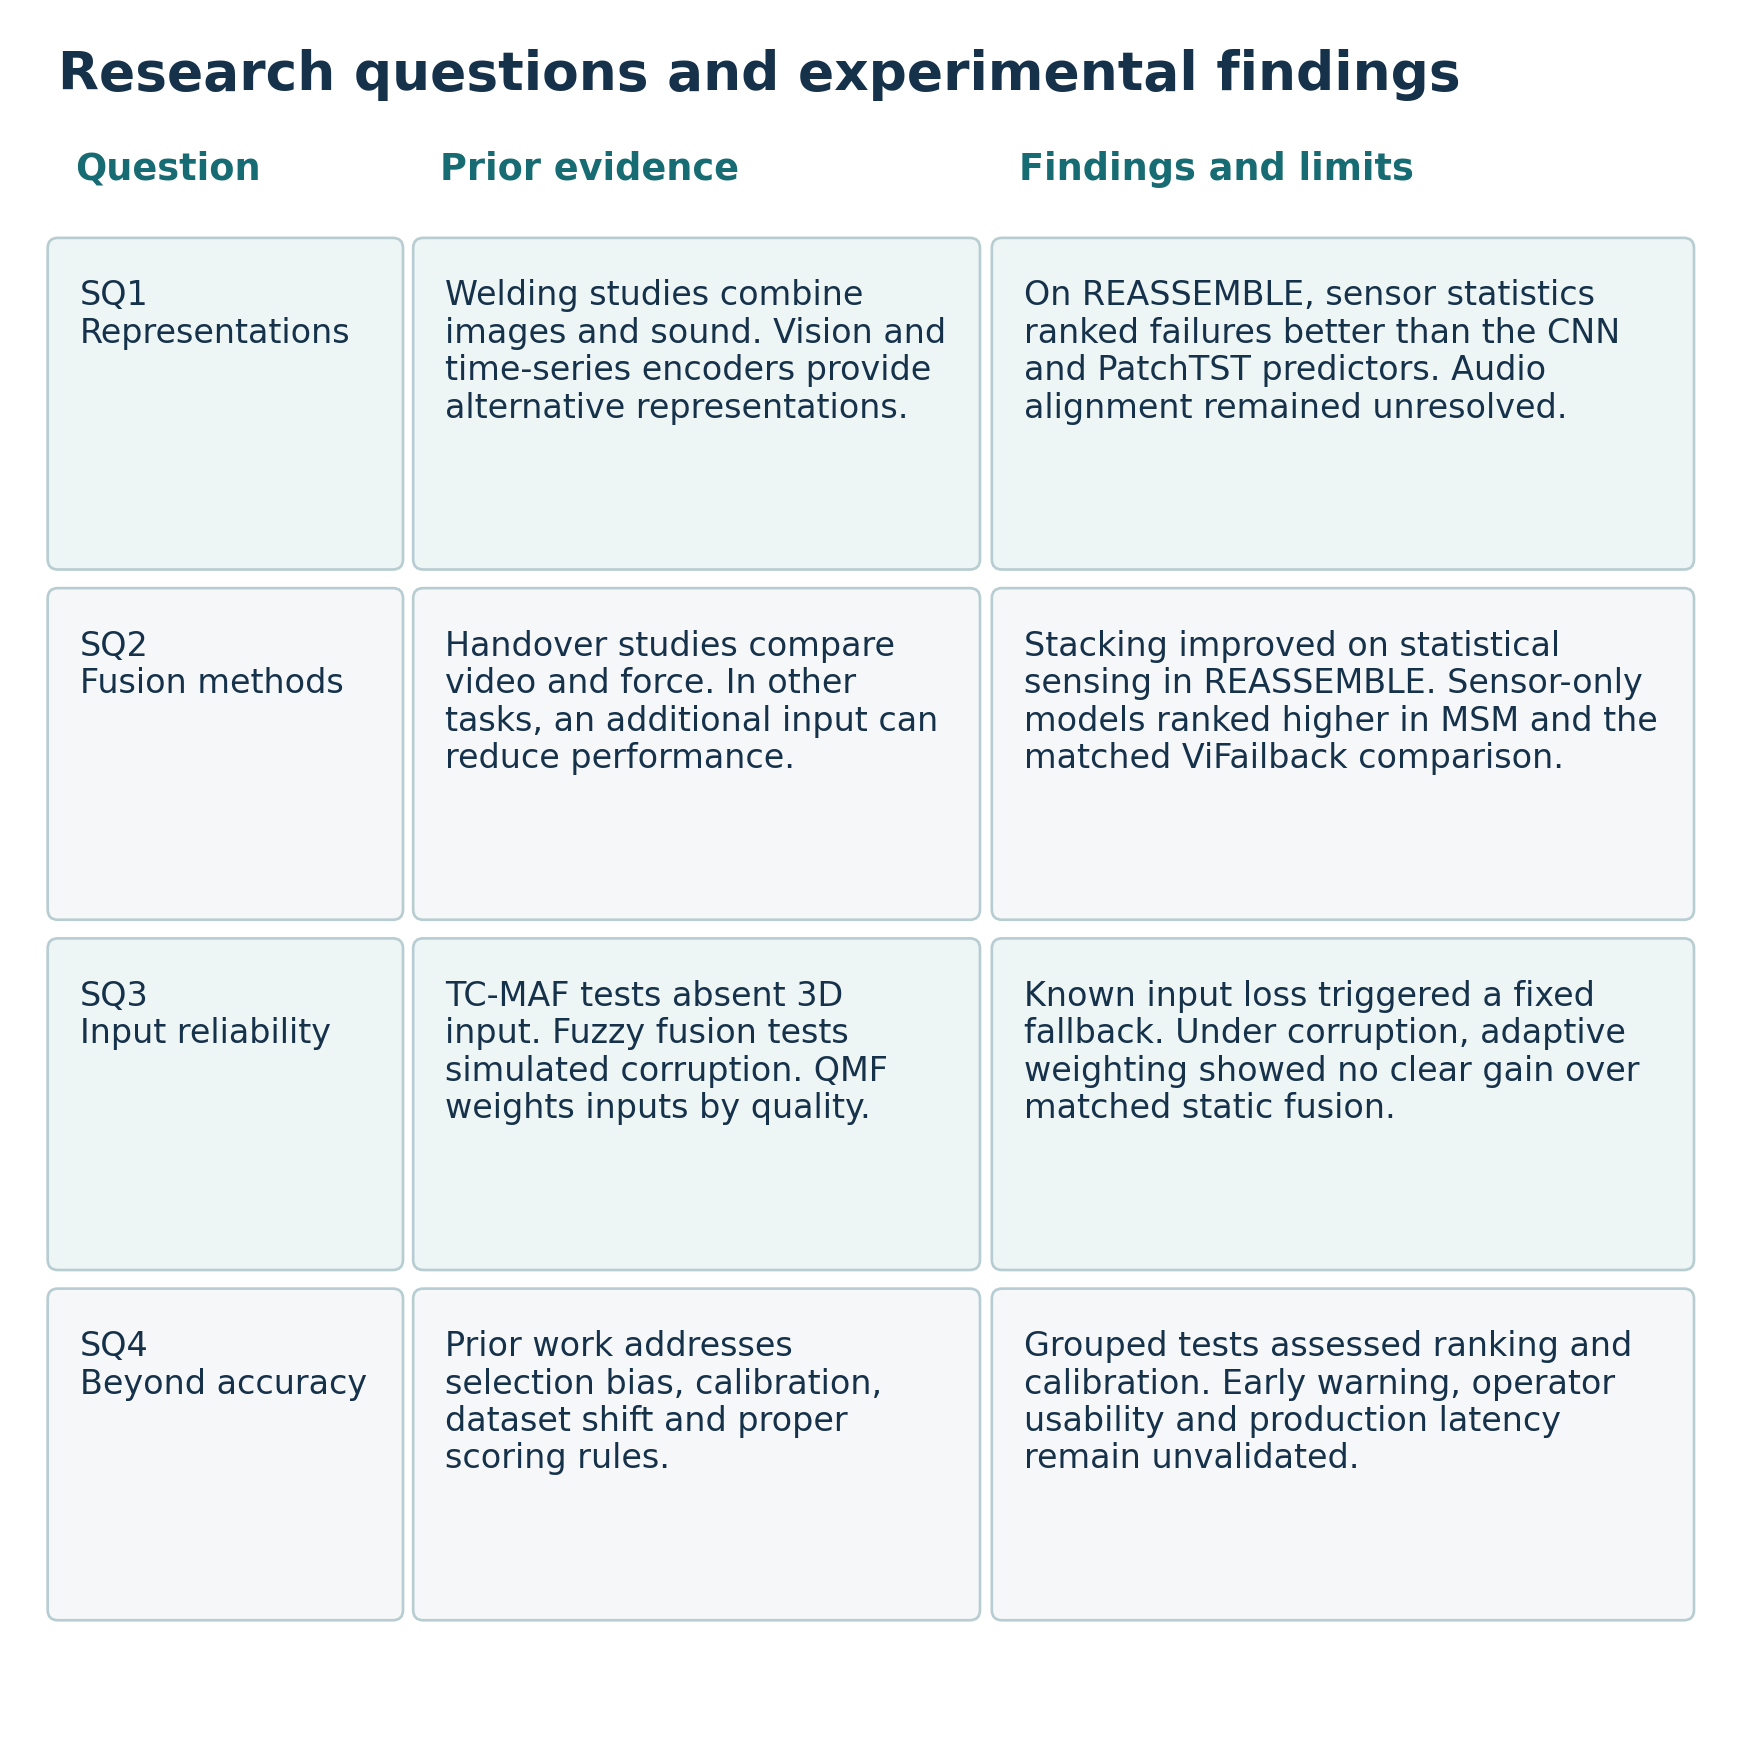
\includegraphics[width=\textwidth]{figures/gap_coverage.png}
\displaynote{The middle column summarizes prior research. The right column gives the corresponding experimental findings and limits.}
\end{figure}

\section{Threats to Validity and Unresolved Evidence}
Three features of the data limit a causal interpretation of architectural differences. First, the target may only approximate the phenomenon of interest. PHM has no independent quantitative tooth-damage reference, MSM's label mapping defines which intervals count as abnormal, and some robotic outcomes remained ambiguous under visual review. Second, the number of independently acquired units can be much smaller than the number of predictions. Gear experiments, recording sessions, dates, tasks, and participants capture different sources of dependence. Where identifiers were missing, independence across those groups could not be verified. Third, several later analyses revisited assessment populations examined during development. Intervals conditional on fitted predictions and variation over a few seeds do not capture that selection history.

Preprocessing before the separate four-arm PHM loop limits attribution of its results to architecture. In other experiments, differences in calibration, capacity, training budget or corruption exposure accompanied architectural changes. Some historical configurations lack the detail needed to reconstruct training exactly. ViFailback evaluated clean predictions from frozen visual backbones. Target-CNN adaptation and corruption effects were outside the final evaluation (Chapter~8). The literature synthesis covers the full texts available to a single reviewer.

Finally, the completed-window studies allowed the predictor to observe evidence near the outcome. Synthetic blur, noise, or stream removal test specified interventions. They give limited information about gradual calibration drift, unobserved timing faults, or shifts to another physical machine. Transferring a predictor to an earlier decision time or a different installation requires observations at that time and place.

\section{Implications for Multimodal System Design}
In a monitoring application, the intended decision determines what constitutes failure, how it can be confirmed independently, and which observations arrive in time to be useful. Evaluating each stream on the same held-out units establishes what it can predict alone. Equal averaging and a fitted static combination then provide references for testing whether context-dependent weights add value. When an instrument declares an outage, the remaining predictor supplies a natural reference. When faulty values still appear plausible, the relevant test is whether the gate recognizes situations in which trusting that stream would worsen the prediction.

A prospective return to welding could reserve whole welding sessions, collect an independent weld-quality measure, and fix the prediction horizon before examining those outcomes. On the same welds, exposure- and calibration-matched models could be assessed for clean performance, known absence, degraded readings, timing error, and shifts between operating conditions. Paired effects and a prespecified tolerance for clean-performance loss would clarify the operational cost of any robustness gain. Such a test would show whether the modest gain for completed assembly actions carries over to weld-quality decisions.
